\begin{figure}[t]
  \centering
  \usetikzlibrary{shapes.arrows, shapes.geometric}
  \definecolor{tak}{HTML}{d3e2ff}
\definecolor{vol}{HTML}{deffb0}
\definecolor{leeg}{HTML}{ffc5b7}

\tikzstyle{terminator}=[rectangle, 
                             draw=black,
                             rounded corners,
                             text centered,
                             minimum height=1.5cm
                            ]
                            
\tikzstyle{choice}=[diamond, 
                             draw=black,
                              rounded corners,
                              text centered,
                              minimum size=1.5cm
                             ]
\tikzstyle{clear}=[rectangle, minimum height=1.55cm, minimum width = 1cm, fill=white]


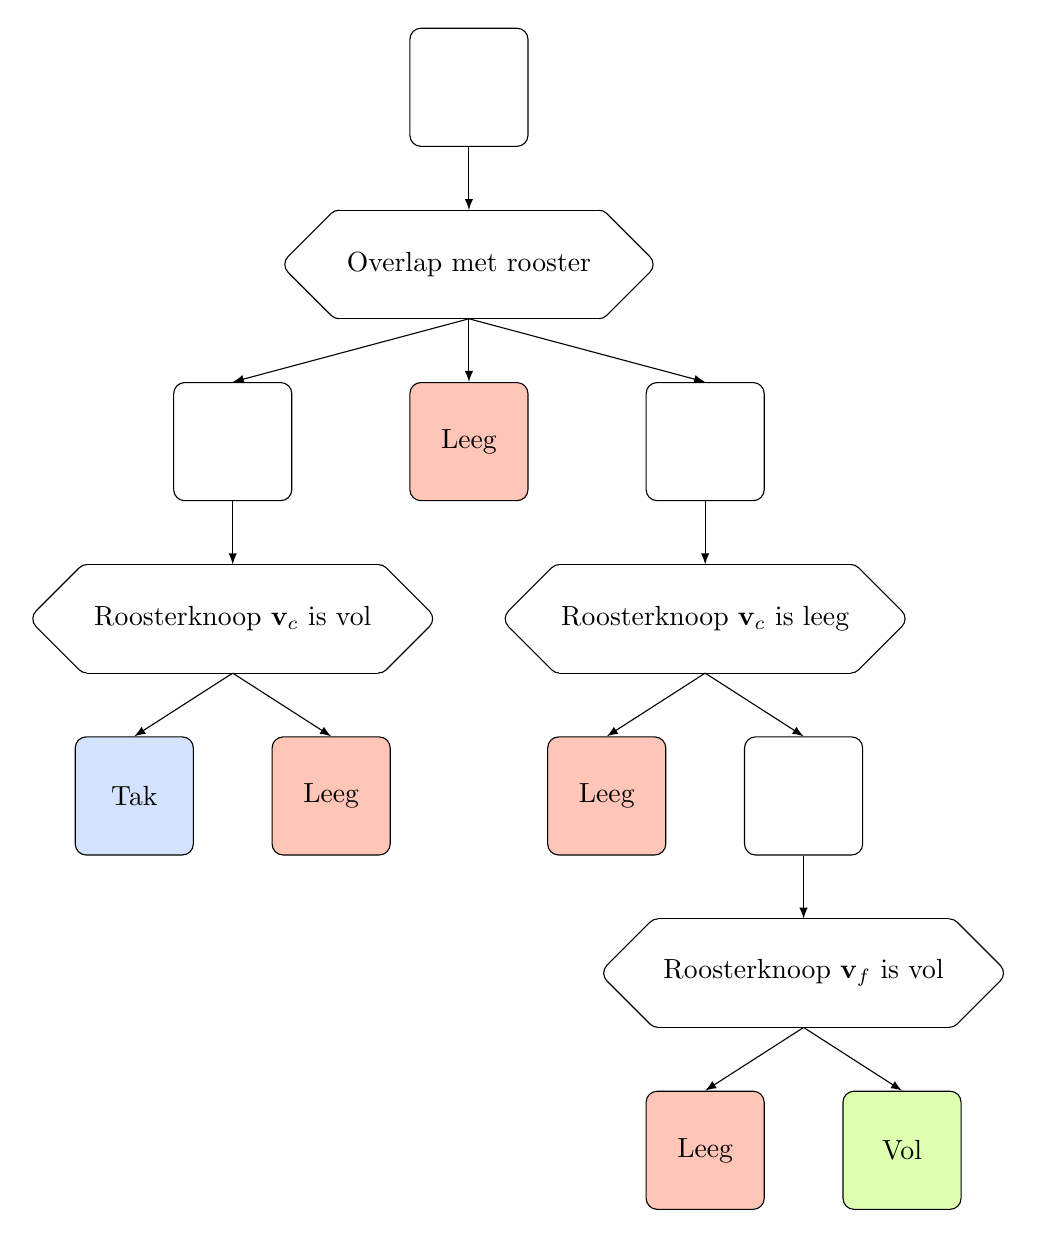
\begin{tikzpicture}
  \node at (0.0cm, 2.25cm) (v) [terminator, minimum width=1.5cm] {};

  \node at ( -1.65cm,  0.0cm) (a) [choice] {};
  \node at ( 1.65cm,  0.0cm) (a) [choice] {};
  \node at ( 0.0cm, 0.0cm) (a) [clear, minimum width=3.3cm] {};
  \node at (-1.65cm, 0.69cm) (ll) {};
  \node at (1.65cm, 0.69cm) (lr) {};
  \draw[-] (ll.center) -- (lr.center) node (up) [pos=0.5] {};
  \node at (-1.65cm, -0.69cm) (ll) {};
  \node at (1.65cm, -0.69cm) (lr) {};
  \draw[-] (ll.center) -- (lr.center) node (down) [pos=0.5] {};
  \node at (0.0cm, 0.0cm) (a) {Overlap met rooster};

\draw[-latex] (v.south) -- (up.center);

  \node at (-3cm, -2.25cm) (v10) [terminator, minimum width=1.5cm] {};
  \node at (0.0cm, -2.25cm) (v11) [terminator, minimum width=1.5cm, fill=leeg] {Leeg};
  \node at (3cm, -2.25cm) (v12) [terminator, minimum width=1.5cm] {};
  
  \draw[-latex] (down.center) -- (v10.north);
  \draw[-latex] (down.center) -- (v11.north);
  \draw[-latex] (down.center) -- (v12.north);

\node at ( -1.85cm -3cm,  0.0cm -4.5cm) (a) [choice] {};
  \node at ( 1.85cm -3cm,  0.0cm -4.5cm) (a) [choice] {};
  \node at ( 0.0cm -3cm, 0.0cm -4.5cm) (a) [clear, minimum width=3.7cm] {};
  \node at (-1.85cm-3cm, 0.69cm -4.5cm) (ll) {};
  \node at (1.85cm-3cm, 0.69cm -4.5cm) (lr) {};
  \draw[-] (ll.center) -- (lr.center) node (up) [pos=0.5] {};
  \node at (-1.85cm-3cm, -0.69cm -4.5cm) (ll) {};
  \node at (1.85cm-3cm, -0.69cm -4.5cm) (lr) {};
  \draw[-] (ll.center) -- (lr.center) node (down) [pos=0.5] {};
  \node at (0.0cm-3cm, 0.0cm -4.5cm) (a) {Roosterknoop $\mathbf{v}_c$ is vol};

\draw[-latex] (v10.south) -- (up.center);

\node at (-4.25cm, -6.75cm) (v20) [terminator, minimum width=1.5cm, fill=tak] {Tak};
\node at (-1.75cm, -6.75cm) (v21) [terminator, minimum width=1.5cm, fill=leeg] {Leeg};

  \draw[-latex] (down.center) -- (v20.north);
  \draw[-latex] (down.center) -- (v21.north);

\node at (1.75cm, -6.75cm) (v30) [terminator, minimum width=1.5cm, fill=leeg] {Leeg};
\node at (4.25cm, -6.75cm) (v31) [terminator, minimum width=1.5cm] {};

\node at ( -1.85cm + 3cm,  0.0cm -4.5cm) (a) [choice] {};
  \node at ( 1.85cm + 3cm,  0.0cm -4.5cm) (a) [choice] {};
  \node at ( 0.0cm + 3cm, 0.0cm -4.5cm) (a) [clear, minimum width=3.7cm] {};
  \node at (-1.85cm + 3cm, 0.69cm -4.5cm) (ll) {};
  \node at (1.85cm + 3cm, 0.69cm -4.5cm) (lr) {};
  \draw[-] (ll.center) -- (lr.center) node (up) [pos=0.5] {};
  \node at (-1.85cm + 3cm, -0.69cm -4.5cm) (ll) {};
  \node at (1.85cm + 3cm, -0.69cm -4.5cm) (lr) {};
  \draw[-] (ll.center) -- (lr.center) node (down) [pos=0.5] {};
  \node at (0.0cm + 3cm, 0.0cm -4.5cm) (a) {Roosterknoop $\mathbf{v}_c$ is leeg};

\draw[-latex] (down.center) -- (v30.north);
  \draw[-latex] (down.center) -- (v31.north);
  \draw[-latex] (v12.south) -- (up.center);

\node at ( -1.85cm + 4.25cm,  0.0cm -9cm) (a) [choice] {};
  \node at ( 1.85cm + 4.25cm,  0.0cm -9cm) (a) [choice] {};
  \node at ( 0.0cm + 4.25cm, 0.0cm -9cm) (a) [clear, minimum width=3.7cm] {};
  \node at (-1.85cm + 4.25cm, 0.69cm -9cm) (ll) {};
  \node at (1.85cm + 4.25cm, 0.69cm -9cm) (lr) {};
  \draw[-] (ll.center) -- (lr.center) node (up) [pos=0.5] {};
  \node at (-1.85cm + 4.25cm, -0.69cm -9cm) (ll) {};
  \node at (1.85cm + 4.25cm, -0.69cm -9cm) (lr) {};
  \draw[-] (ll.center) -- (lr.center) node (down) [pos=0.5] {};
  \node at (0.0cm + 4.25cm, 0.0cm -9cm) (a) {Roosterknoop $\mathbf{v}_f$ is vol};

\draw[-latex] (v31.south) -- (up.center);

\node at (3cm, -11.25cm) (v40) [terminator, minimum width=1.5cm, fill=leeg] {Leeg};
\node at (5.5cm, -11.25cm) (v41) [terminator, minimum width=1.5cm, fill=vol] {Vol};
\draw[-latex] (down.center) -- (v40.north);
  \draw[-latex] (down.center) -- (v41.north);
\end{tikzpicture}
  \caption{De beslissingsboom om het type van een octreeknoop te bepalen.}
  \label{fig:hs-licht-octree-dt}
\end{figure}
